\documentclass[
	% handout
]{beamer}
\setbeamertemplate{navigation symbols}{}
\usepackage{xcolor}
\definecolor{seeblau}{HTML}{00A9E0}
\definecolor{seegrau}{HTML}{9AA0A7}

\definecolor{seeblau1}{HTML}{CCEEF9}
\definecolor{seeblau2}{HTML}{A6E1F4}
\definecolor{seeblau3}{HTML}{59C7EB}
\definecolor{seeblau4}{HTML}{00A9E0}
\definecolor{seeblau5}{HTML}{008ECE}

\setbeamercolor{title}{fg=seeblau}
\setbeamercolor{frametitle}{fg=seeblau}
\setbeamercolor{section in toc}{fg=seeblau}
\setbeamercolor{structure}{fg=seeblau}

\setbeamertemplate{footline}{%
	\begin{beamercolorbox}[sep=1em,wd=\paperwidth,leftskip=0.5cm,rightskip=0.5cm]{footlinecolor}
		\small\textbf{\insertsection}\quad\insertsubsection\hfill\insertframenumber
	\end{beamercolorbox}%
}

\usepackage[english]{babel}
\parskip=20pt

\usepackage[sfdefault]{roboto}
\usepackage{sfmath}

\usepackage{ifthen, adjustbox}
\newcommand{\markieren}[4]{
	\ifthenelse{\equal{#1}{}}{}{\adjustbox{padding=3pt, bgcolor=seeblau1, margin=-1pt}{\strut{\sffamily\robotoMedium{#1}}}\\}
  \ifthenelse{\equal{#2}{}}{}{\adjustbox{padding=3pt, bgcolor=seeblau2, margin=-1pt}{\strut{\sffamily\robotoMedium{#2}}}\\}
	\ifthenelse{\equal{#3}{}}{}{\adjustbox{padding=3pt, bgcolor=seeblau3, margin=-1pt}{\strut{\sffamily\robotoMedium{#3}}}\\}
	\ifthenelse{\equal{#4}{}}{}{\adjustbox{padding=3pt, bgcolor=seeblau4, margin=-1pt}{\strut{\sffamily\robotoMedium{#4}}}}
}

\usepackage[
	style=authortitle
]{biblatex}
\newcommand{\customcite}[1]{
\let\thefootnote\relax\footnotetext{
	\tiny\raggedleft
	\emph{\citetitle{#1}}, \citeauthor*{#1} \citeyear{#1}
}
}


\usepackage[ddmmyyyy]{datetime}
\renewcommand{\dateseparator}{.}

\usepackage{amsmath,amssymb,amsfonts,amsthm}

\addbibresource{literature.bib} 
\DeclareMathOperator{\Tr}{Tr}

\author{Leon Oleschko}
\institute{Universität Konstanz}
\date{31.01.2025}

\begin{document}
{
\setbeamertemplate{footline}{} 
\begin{frame}
	\huge
	\markieren{}{Quantum Measurement}{Zeno Effect}{Standard Quantum Limit}
	
	\vfill
	\normalsize
	Leon Oleschko\\
	\today
	
	\vfill
	\raggedleft
	\small
	\textit{Modeling Quantum Hardware: open dynamics and control}\\
	Universität Konstanz
\end{frame}
}

\begin{frame}{}
	\Large
	No phenomenon is a real until it is observed.\\
	\normalsize\raggedleft
	 -- John A. Wheeler 1970
\end{frame}

\begin{frame}{Historical Note}
	\begin{itemize}
		\item[1900] Plank \& Einstein: Blackbody Radiation
		\item[1920] Bohr, Heisenberg: Copenhagen interpretation\\
		Born: Probabilistic interpretation $P(m) = |\langle m| \psi \rangle|^2$\\
		Schrödinger: Measurement Problem 
		\item[1930] EPR Paradox
		\item[1932] von Neumann: \textit{Mathematical Foundations of Quantum Mechanics}
		\item[1970] Decoherence Theory
		\item[present] Experimental Interest
	\end{itemize}
\end{frame}


\section{Strong Measurement}
\begin{frame}{Projective (von Neumann) Measurement}
	Measurement Operator $\hat A = \sum m |m\rangle$ on $\psi$:
	$$p(m) = |\langle m|\psi\rangle|^2$$
	$$\psi \xrightarrow{\text{Measuring }m} |m\rangle$$

	More formally with projector $\hat M \sim |m\rangle\langle m|$:
	$$\rho' \propto \hat M \rho \hat M$$

	{\small\textcolor{seegrau}{
		Neglegting Normalization and Degenercy:
		POVM Measurement
	}}

	\customcite[2.2.3]{nielsen_quantum_2010}
	\highlightcite[1]{wiseman_quantum_2010}
\end{frame}

\begin{frame}{Example: Superposition}
	\begin{columns}
		\column{.5\textwidth}
		\begin{align*}
			H &= \sigma_z\\
			|\psi> &\propto |\uparrow\rangle + |\downarrow\rangle\\
			i \partial_t \psi &= H \psi
		\end{align*}
		$\Rightarrow$ Superposition is stable

		\only<2>{
			$$M = \sigma_z$$
			$$p(\updownarrow)=|\langle\updownarrow|\psi\rangle|^2 = \frac{1}{2}$$
		}


		\column{.5\textwidth}
		\centering
		\only<1>{
			\includegraphics{figures/03 free.pdf}
		}
		\only<2>{
			\includegraphics{figures/03 measurement.pdf}
		}
	\end{columns}
\end{frame}

\begin{frame}{Example: Decay}
	\begin{columns}
		\column{.2\textwidth}
		\begin{align*}
			H &= \sigma_z\\
			|\psi> &\propto |\uparrow\rangle\\
			M &= \sigma_z\\
			J &= \kappa\sigma_-\\
			\partial_t\rho &= -i [H, \rho] \\
			&+ J\rho J^\dagger - \frac{1}{2} \{J^\dagger J, \rho\} 
		\end{align*}
		
		\column{.8\textwidth}
		\centering
		\vspace{-1cm}
		\includegraphics{figures/04 discreate.pdf}
	\end{columns}
\end{frame}

\begin{frame}{Example: Zeno}
	\centering
	\includegraphics{figures/04 discreate zeno.pdf}
\end{frame}

\begin{frame}{Zeno Effect}
	\begin{columns}
		\column{.6\textwidth}
		\begin{itemize}
			\item<1-> Zeno of Elea (460 BCE): Arrow paradox
			\item<1-> Misra and Sudarshan (1977): “The Zeno's paradox in quantum theory”
			\item<2-> Experimentally demonstrated (1990) with 5000 $^9$Be$^+$ ions at 250 mK
			\item<3-> Used in Magnetometers and possibly birds
		\end{itemize}
		\only<3->{\customcite{kominis_quantum_2009}}

		\column{.4\textwidth}
		\centering
		\only<2->{
			\includegraphics[width=\textwidth]{figures/zeno_energy.png}
			\includegraphics[width=.8\textwidth]{figures/zeno_data.png}
			\highlightcite{itano_quantum_1990}
		}
	\end{columns}
\end{frame}

\begin{frame}{Practical Examples of strong measurements}
	\begin{columns}
		\column{.5\textwidth}
		\begin{itemize}
			\item<1-> Trapped Ions
			\item<2-> Superconducting Qubits
			\item<3-> Stern-Gerlach Experiment
			\item<4-> Quantum Dot Charge Readout
		\end{itemize}

		\column{.5\textwidth}
		\only<1>{\includegraphics[width=\textwidth]{figures/zeno_energy.png}}
		\only<2>{\includegraphics[width=\textwidth]{figures/qubit_circuit.jpg}}
		\only<3>{\includegraphics[width=\textwidth]{figures/stern-gerlach.jpg}}
		\only<4>{\includegraphics[width=\textwidth]{figures/qd_charge.png}}
		\only<5>{
			$\Rightarrow$ 
			Used when the quantum wave function is collapsed into a classical result
			\vspace{1em}

			\begin{itemize}
				\item measurement of conjugate variables
				\item optical measurements
				\item Continuous measurement not possible
			\end{itemize}
			\customcite[]{wiseman_quantum_2010}
		}
	\end{columns}
	
\end{frame}

\section{Weak Measurement}
\begin{frame}{Weak Measurement}
	\begin{center}
		\includegraphics{figures/back_action.pdf}
	\end{center}
	$$H = H_S\otimes 1 + 1\otimes H_M + g(t) \; C_S \otimes P_M$$
	
	measuring $\hat X$ in $M$: $\langle C\rangle + \xi_g$ and partial collapse in $S$

	Continuous application leads to \emph{SME} for $S$:
	$$
		\partial_t\rho 
		= -i[H,\rho] 
		+ J\rho J^\dagger - \frac{1}{2} \{J^\dagger J, \rho\} 
		+ \left(C\rho + \rho C^\dagger - \Tr(C\rho + \rho C^\dagger)\right)\xi(t)
	$$

	\customcite[Fig 8.4 modified]{vladimir_braginsky_quantum_1992}
	\highlightcite[]{jacobs_straightforward_2006}
\end{frame}

% Measurement Operator $\hat M = \sum m |m\rangle$ on $\psi$:
% $$p(m) = |\langle m|\psi\rangle|^2$$
% $$\psi \xrightarrow{\text{Measuring }m} |m\rangle$$


% \begin{frame}{Kraus Operators}
% 	Measuring $A = \sum a |a\rangle$ define Kraus operators:
% 	$$
% 		K_0 = \sqrt{1-p}\; I,  \quad
% 		K_a = \sqrt{p} \; | a \rangle\langle a |
% 	$$

% 	Evolution after stochastically choosing $a$:
% 	$$\rho\rightarrow K_m \rho K^\dagger_m$$

% 	Measuring Result: $$a + \frac{\mathcal{N}(1)}{\sqrt{p}}$$

% 	\customcite[]{clerk_introduction_2010}
% \end{frame}

\begin{frame}{Example: Weak measurement}
	\begin{columns}
		\column{.2\textwidth}
		\begin{align*}
			H &= \sigma_z\\
			\psi &= \uparrow\\
			M &= \sigma_z\\
			J &= \kappa\sigma_-\\
			C &= \eta \sigma_z
		\end{align*}


		\column{.8\textwidth}
		\centering
		\includegraphics{figures/06 sme.pdf}
	\end{columns}
\end{frame}


\begin{frame}{Practical Examples of weak measurements}
	\begin{columns}
		\column{.5\textwidth}
		\begin{itemize}
			\item continuous measurements\\
			\item<2-> feedback control
			\item<3-> state tomography
		\end{itemize}
		
		\column{.5\textwidth}
		\only<1>{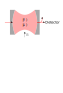
\includegraphics[width=\textwidth]{figures/rabi.pdf}}
		\only<2>{\includegraphics[width=\textwidth]{figures/feedback.png}}
		\only<3>{\includegraphics[width=\textwidth]{figures/stateTomography.png}}
	\end{columns}
\end{frame}

\begin{frame}{Interferometer and SQL}
	\begin{columns}
		\column{0.5\textwidth}
		\centering
		\includegraphics{figures/drawing.pdf}
		\only<2->{\includegraphics[width=\textwidth]{figures/sub_sql.png}}
		
		\column{0.5\textwidth}
		\includegraphics[width=\textwidth]{figures/Fig 1.png}
	\end{columns}

	\customcite[]{braginskit_quantum-mechanical_1974}
	\customcite[]{teufel_nanomechanical_2009}
	\customcite[]{tse_quantum-enhanced_2019}
\end{frame}

\begin{frame}{}
	\begin{columns}
		\column{.4\textwidth}
		\includegraphics[width=\textwidth]{figures/04 discreate zeno.pdf}
		\includegraphics[width=\textwidth]{figures/06 sme small.pdf}
		
		\column{.4\textwidth}
		\includegraphics{figures/drawing.pdf}
		\includegraphics[width=\textwidth]{figures/sub_sql.png}
	\end{columns}

\end{frame}

% \begin{frame}{Example: Real System}
% 	\begin{columns}
% 		\column{.5\textwidth}
% 		\begin{center}
% 			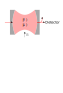
\includegraphics{figures/rabi.pdf}
% 		\end{center}

% 		\column{.5\textwidth}
% 		\begin{align*}
% 			H &= \sigma_z &\text{Atom}\\
% 			&+ a^\dagger a + g \sigma_z a^\dagger a &\text{M}\\
% 			J &= \kappa\; a &\text{Dissipation}\\
% 			C &= \kappa\eta\; a &\text{Measurement}
% 		\end{align*}
		
% 	\end{columns}

% 	\customcite{nielsen_stochastic_2008}
% \end{frame}


% \begin{frame}{Rabi Oscillations Setup}
% 	\begin{columns}
% 		\column{.5\textwidth}
% 		\begin{center}
% 			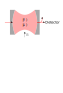
\includegraphics{figures/rabi.pdf}
% 		\end{center}

% 		\column{.5\textwidth}
% 		\begin{align*}
% 			H &= g\; (a^\dagger a) (\sigma^+ \sigma^-) &\text{Coupling}\\
% 			&+ g_s\; (\sigma^+ + \sigma^-) &\text{Magnetic}\\
% 			&- i \beta (a^\dagger - a) &\text{Optic}\\
% 			J &= \kappa\; a &\text{Dissipation}\\
% 			C &= \sqrt{\kappa\eta}\; a &\text{Measurement}
% 		\end{align*}
		
% 	\end{columns}

% 	\customcite{nielsen_stochastic_2008}
% \end{frame}

% \begin{frame}{Time evolution}
% 	\includegraphics{figures/02 rabi w measurement.pdf}
% \end{frame}


{
	\setbeamercolor{background canvas}{bg=black}
	\begin{frame}[plain]{}\end{frame}
}

\begin{frame}{Types of Measurements}
	\begin{columns}
		\column{.5\textwidth}
		\includegraphics[width=\textwidth]{figures/types_table.png}

		\column{.5\textwidth}
		\includegraphics[width=\textwidth]{figures/types_ven.png}
	\end{columns}
	\customcite{wiseman_quantum_2010}
\end{frame}

\section{Standard Quantum Limit}
\input{notes_sql.tex}

\end{document}
